\documentclass[12pt,lithuanian,]{article}
\usepackage{lmodern}
\usepackage{amssymb,amsmath}
\usepackage{ifxetex,ifluatex}
\usepackage{fixltx2e} % provides \textsubscript
\ifnum 0\ifxetex 1\fi\ifluatex 1\fi=0 % if pdftex
  \usepackage[T1]{fontenc}
  \usepackage[utf8]{inputenc}
\else % if luatex or xelatex
  \ifxetex
    \usepackage{mathspec}
  \else
    \usepackage{fontspec}
  \fi
  \defaultfontfeatures{Ligatures=TeX,Scale=MatchLowercase}
\fi
% use upquote if available, for straight quotes in verbatim environments
\IfFileExists{upquote.sty}{\usepackage{upquote}}{}
% use microtype if available
\IfFileExists{microtype.sty}{%
\usepackage{microtype}
\UseMicrotypeSet[protrusion]{basicmath} % disable protrusion for tt fonts
}{}
\usepackage[margin=1in]{geometry}
\usepackage{hyperref}
\hypersetup{unicode=true,
            pdftitle={Bajeso FAVAR-TVP modelio taikymas JAV ekoniminiams ir rinkos duomenims},
            pdfauthor={Gediminas Bagdonas \textless{}gediminas.bagdonas@mif.vu.lt\textgreater{}},
            pdfborder={0 0 0},
            breaklinks=true}
\urlstyle{same}  % don't use monospace font for urls
\ifnum 0\ifxetex 1\fi\ifluatex 1\fi=0 % if pdftex
  \usepackage[shorthands=off,main=lithuanian]{babel}
\else
  \usepackage{polyglossia}
  \setmainlanguage[]{lithuanian}
\fi
\usepackage{natbib}
\bibliographystyle{plainnat}
\usepackage{longtable,booktabs}
\usepackage{graphicx,grffile}
\makeatletter
\def\maxwidth{\ifdim\Gin@nat@width>\linewidth\linewidth\else\Gin@nat@width\fi}
\def\maxheight{\ifdim\Gin@nat@height>\textheight\textheight\else\Gin@nat@height\fi}
\makeatother
% Scale images if necessary, so that they will not overflow the page
% margins by default, and it is still possible to overwrite the defaults
% using explicit options in \includegraphics[width, height, ...]{}
\setkeys{Gin}{width=\maxwidth,height=\maxheight,keepaspectratio}
\IfFileExists{parskip.sty}{%
\usepackage{parskip}
}{% else
\setlength{\parindent}{0pt}
\setlength{\parskip}{6pt plus 2pt minus 1pt}
}
\setlength{\emergencystretch}{3em}  % prevent overfull lines
\providecommand{\tightlist}{%
  \setlength{\itemsep}{0pt}\setlength{\parskip}{0pt}}
\setcounter{secnumdepth}{5}
% Redefines (sub)paragraphs to behave more like sections
\ifx\paragraph\undefined\else
\let\oldparagraph\paragraph
\renewcommand{\paragraph}[1]{\oldparagraph{#1}\mbox{}}
\fi
\ifx\subparagraph\undefined\else
\let\oldsubparagraph\subparagraph
\renewcommand{\subparagraph}[1]{\oldsubparagraph{#1}\mbox{}}
\fi

%%% Use protect on footnotes to avoid problems with footnotes in titles
\let\rmarkdownfootnote\footnote%
\def\footnote{\protect\rmarkdownfootnote}

%%% Change title format to be more compact
\usepackage{titling}

% Create subtitle command for use in maketitle
\newcommand{\subtitle}[1]{
  \posttitle{
    \begin{center}\large#1\end{center}
    }
}

\setlength{\droptitle}{-2em}
  \title{Bajeso FAVAR-TVP modelio taikymas JAV ekoniminiams ir rinkos duomenims}
  \pretitle{\vspace{\droptitle}\centering\huge}
  \posttitle{\par}
  \author{Gediminas Bagdonas
\textless{}\href{mailto:gediminas.bagdonas@mif.vu.lt}{\nolinkurl{gediminas.bagdonas@mif.vu.lt}}\textgreater{}}
  \preauthor{\centering\large\emph}
  \postauthor{\par}
  \predate{\centering\large\emph}
  \postdate{\par}
  \date{2017-02-16}

\usepackage{float}
\usepackage[tableposition=top]{caption}
\usepackage{setspace}
\usepackage{indentfirst}

\hypersetup{
  colorlinks=true,
  urlcolor=blue,
  linkcolor=red,
  citecolor=blue,
  allbordercolors={0 0 0},
  pdfborderstyle={/S/U/W 1}
}
\setlength\parindent{24pt}\setlength{\parskip}{0.0pt plus 1.0pt}
\onehalfspacing

\begin{document}
\maketitle

\section{Užduotis}\label{uzduotis}

Rasti modelį, kuris susietų JAV ekonominius duomenis ir JAV vyriausybės
vertybinių popierių (VVP) pajamingumų kreivę. Ištirti ekonominių duomenų
įtaką pajamingumų kreivės formai ir rasti sąlygines prognozes
skirtingiems ekonominiams scenarijams.

\section{Duomenys}\label{duomenys}

Naudojame ketvirtinius duomenis nuo 1967K2 iki 2016K4. Tyrimui naudojame
šias laiko eilutes:

\begin{itemize}
\tightlist
\item
  \texttt{UNRATE} - JAV nedarbo lygis. Asmenys vyresni nei 16 metų,
  neturintys darbo, galintys bei pasirengę dirbti ir aktyviai ieškantys
  darbo. Procentiniais punktais nuo visos darbo jėgos. Pakoreguotas
  atsižvelgiant į sezoniškumą.
\item
  \texttt{CPILFESL} - JAV infliacijos lygis procentiniais punktais.
  Visos vartojimo prekės išskyrus maisto ir energetikos sektorius.
  Pakoreguotas atsižvelgiant į sezoniškumą.
\item
  \texttt{GDPC1} - realus (atėmus infliaciją) BVP. Metinis pokytis
  procentiniais punktais. Pakoreguotas atsižvelgiant į sezoniškumą.
\item
  \texttt{SVENPY{[}x{]}} - {[}x{]} metų trukmės JAV vyriausybės
  obligacijų pajamingumo norma procentiniais punktais.
\end{itemize}

Ekonominius duomenis galima rasti St.~Louis Fed puslapyje
(\url{https://fred.stlouisfed.org}). Pajamingumo kreivių šaltinis:
Federal Reserve (\url{http://www.federalreserve.gov/pubs/feds/2006}).

Naudotos laiko eilutės pateiktos \ref{fig:data} Pav. Dešinėje
pavaizduoti ekonominiai duomenys, o kairėje keli pajamingumų kreivės
taškai.

\begin{figure}[htbp]
\centering
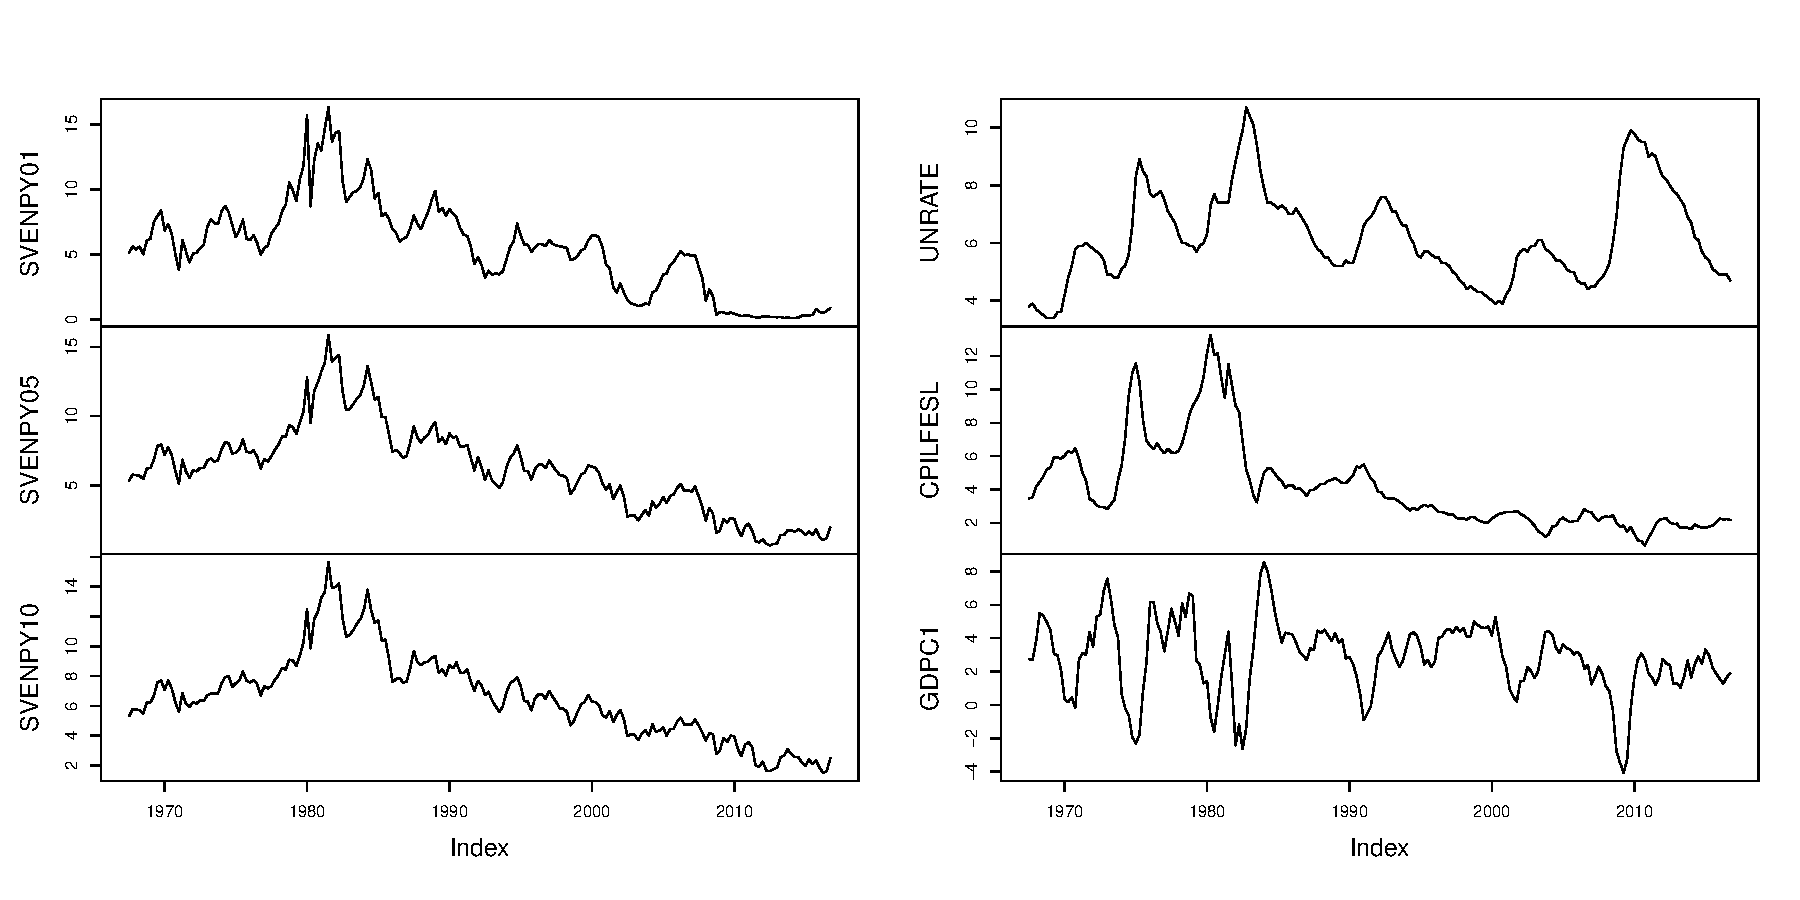
\includegraphics{bayesFAVAR_TVP_files/figure-latex/data-1.pdf}
\caption{\label{fig:data}Nagrinėjamų ekonominių ir rinkos rodiklių
istoriniai duomenys}
\end{figure}

\subsection{Pajamingumo kreivė}\label{pajamingumo-kreive}

Skirtingų trukmių vertybinų popierių pajamingumai yra stipriai
koreliuoti (žr. \ref{fig:data} Pav) ir tipiškai didėja, didėjant trukmei
iki išpirkimo. Skirtingų trukmių obligacijų gali būti daug, todėl dažnai
modeliuojant naudojama pajamingumų kreivė, kuri nusako pajamingumo normą
skirtingos trukmės vertybiniams popieriams. Tipinę kreivės formą galima
pamatyti \ref{fig:yc_example} pav. Mes analizėje naudojame 1, 2,
\ldots{}, 10 metų fiksuotus kreivės taškus.

\begin{figure}[htbp]
\centering
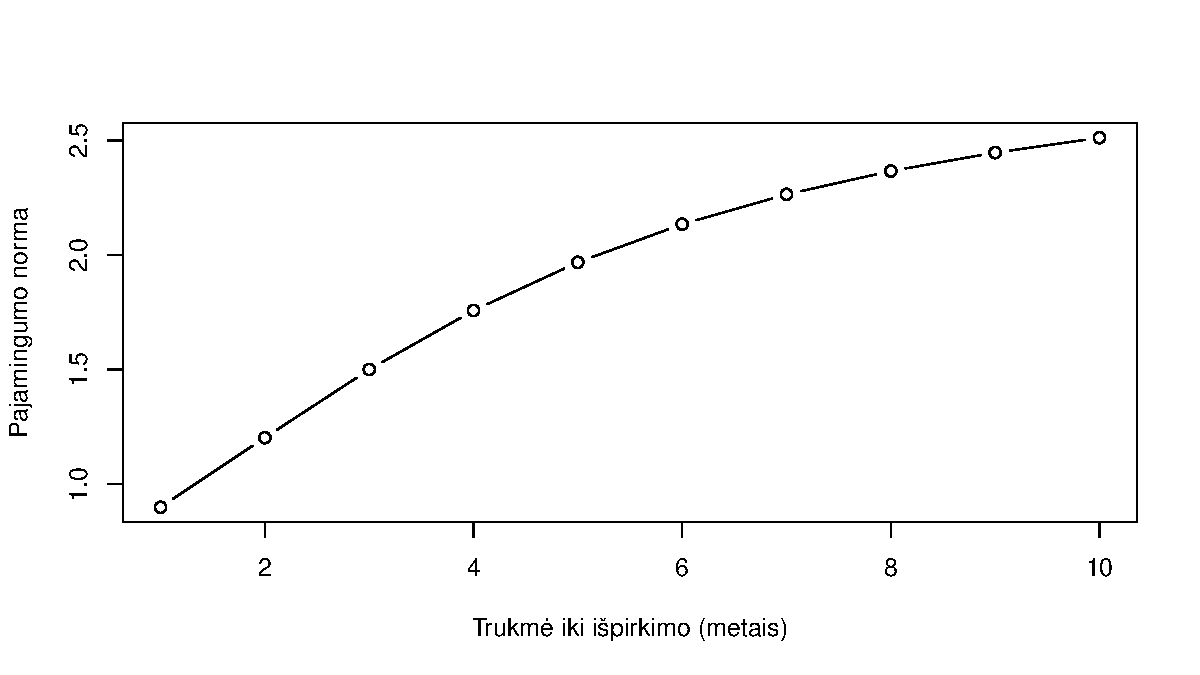
\includegraphics{bayesFAVAR_TVP_files/figure-latex/yc_example-1.pdf}
\caption{\label{fig:yc_example}JAV VP pajamingumo kreivė}
\end{figure}

Dažnai pajamingumo kreivė yra aprašoma trimis faktoriais: lygiu, statumu
ir kreivumu. Pvz. \citet{NelsonSiegel} pasiūlė tokį kreivės faktorių
išskyrimą:

\[ y_t(m) = \beta^L_t + \beta^S_t \left(\frac{1-\exp(-m \lambda)}{m\lambda}\right) + \beta^C_t \left(\frac{1-\exp(-m \lambda)}{m\lambda} - \exp(-m \lambda)\right).\]
Čia \(m\) žymi trukmę iki obligacijos išpirkimo, \(y_t\) - pajamingumo
lygį, o \(\lambda\) parametras, kuris nusako kurioje kreivės vietoje
maksimizuojamas kreivumas. Tai maždaug atitinka PCA rezultatus (pirmos
trys didžiausios variacijos komponentės). Tokia praktika motyvavo FAVAR
modelio pasirinkimą.

\section{Trumpai apie TVP-FAVAR
modelį}\label{trumpai-apie-tvp-favar-modeli}

Analizei pasirinkome faktoriais papildytą vektorinės autoregresijos su
laike kintančiais parametrais modelį (TVP-FAVAR). Tokį pasirinkimą lėmė
keli veiksniai. Kaip minėjome visą pajamingumo kreivę gan gerai aprašo
trys faktoriai. Kita vertus, kadangi nagrinėjome ilgą laikotarpį yra gan
realu, kad per tą laikotarpį ekonominiai sąryšiai galėjo kisti, todėl
pasirinkome modelį su laike kintančiais parametrais. Modelis užrašomas
trimis lygtimis:

\[ y_t = \Lambda F_t + r_t; \qquad r_t \sim N(0, R) \]
\[ F_t = Z_t \beta_t + \epsilon_t; \qquad \epsilon_t \sim N(0, H) \]
\[ \beta_{t+1} = \beta_t + u_t; \qquad u_t \sim N(0, Q),\] \(Z_t\) žymi
matricą \[ Z_t = [1, F_{t-1}, F_{t-2}, ..., F_{t-p}] \otimes I_n \] Mūsų
nagrinėjamu atveju
\[ y_t = (\text{SVENPY01}_t, ..., \text{SVENPY10}_t, \text{UNRATE}_t, \text{CPILFESL}_t, \text{GDPC1}_t), \]
\[ F_t = (F^1_t, F^2_t, F^3_t, \text{UNRATE}_t, \text{CPILFESL}_t, \text{GDPC1}_t), \]
ir \[ \Lambda = \left( \begin{array}{cccccc}
\lambda_{1;1} & \lambda_{1;2} & \lambda_{1;3} & 0 & 0 & 0 \\
... & ... & ... & ... & ... & ... \\
\lambda_{10;1} & \lambda_{10;2} & \lambda_{10;3} & 0 & 0 & 0 \\
0  & 0 & 0 & 1 & 0 & 0 \\
0  & 0 & 0 & 0 & 1 & 0 \\
0  & 0 & 0 & 0 & 0 & 1 \\
\end{array} \right). \] Taip pat darome prielaidą, kad \(R\) diagonalinė
matrica (visa tarpusavio priklausomybė atsiranda tik iš fakorių).

\subsection{Apriori skirstiniai}\label{apriori-skirstiniai}

Parametrams \(\Lambda\) ir \(R\) pasirinkome Normalųjų-Atvirkštinį Gama
(angl. \emph{normal-inverse gamma}) priorą, kadangi laikant kitus
parametrus žinomais pirma lygtis nusako tiesinės regresijos modelį. Šiuo
atveju pasirinkome

\[R_{ii} \sim IG(0.01, 1); \qquad \lambda_{ij} \sim N(0, 1).\] \(F_t\)
ir \(\Lambda\) pradinės reikšmės gautos iš PCA, tačiau išmėginome ir
kitas pradines reikšmes.

Modelio parametrams \(\beta_0\), \(H\) ir \(Q\) pasirinkome patogų ir
gan bendrą nepriklausomą Normalųjų-Wishart (angl. \emph{independent
Normal-Wishart}) apriorinį skirstinį, t.y.
\[ p(\beta_1, H^{-1}, Q^{-1}) = p(\beta_1) p(H^{-1}) p(Q^{-1}), \] kur
\[\beta_1 \sim N(\underline{\beta}, \underline{V}_{\beta}) ,\]
\[H^{-1} \sim W(\underline{S}^{-1}, \underline{\nu}), \]
\[Q^{-1} \sim W(\underline{Q}^{-1}, \underline{\nu}_Q). \]

Apriorų hiperparametrų nustatymui sekėme \citet{Primiceri2005} ir juos
pasirenkome naudodami OLS sprendinį pirmiems 40 stebėjimų
(\(\tau = 40\)), t.y. nuo 1967K2 iki 1977K1. Pats FAVAR-TVP modelio
skaičiavimas pradedamas nuo 1977K2. Hiperparametrai nustatomi naudojant
OLS sprendinį \(\beta_{OLS}\) ir kovariacijų matricą \(V(\beta_{OLS})\).
Šiam tyrimui pasirinkome
\[\underline{\beta} = \beta_{OLS}; \quad \underline{V}_{\beta} = 4V(\beta_{OLS}); \quad  \underline{\nu} = n +1; \quad \underline{S} = I_n; \quad \underline{\nu}_Q = \tau; \quad \underline{Q} = 10^{-6} \tau V(\beta_{OLS})\]
Reiktų pastebėti, kad pasirinkome labai mažas kovariacijas matricoje
\(\underline{Q}\). Tai atspindi mūsų a priori požiūrį, kad parametrai
\(\beta_t\) turėtų būti mažai kintantys.

Nepriklausomas normaliojo-Wishart bei normaliojo-atv. gama aprioras
leidžia sukonstruoti paprastą MCMC algoritmą, kuris paeiliui generuoja
\(p(\beta_1 | F_T, \beta_T, H)\), \(p(H^{-1}| F_T, \beta_1, \beta_T)\),
\(p(Q^{-1}|F_T, \beta_1, \beta_T )\),
\(p(\beta_T |F_T, \beta_1, H, Q)\), \(p(\Lambda | y_T, F_T, R)\),
\(p(R| y_T, F_T, \Lambda)\) ir \(p(F_T|y_T, R, \Lambda, H)\). Plačiau
apie MCMC algoritmą galima rasti \citet{KoopKorobilis2010},
\citet{blake2012applied}, \citet{Bernanke2004} ir
\citet{EllisMumtaz2014}.

Verta paminėti, kad yra keliatas algoritmų skirtų
\(p(\beta_T | F_T, \beta_1, H, Q)\) generavimui. Mes išmėginome du iš jų
\citet{CC1994} ir \citet{DK2002}. Abu algoritmai grąžina panašius
rezultatus, tačiau mūsų \citet{DK2002} implementacija veikia šiek tiek
greičiau.

Kita a priori prielaida modeliuojant ekonominius duomenis dažnai yra,
kad nagrinėjamos laiko eilutės yra stacionarios. Mes taip pat darome šią
prielaidą ir ją implementuojame, naudodami priėmimo-atmetimo (angl.
\emph{accept-reject}) žingsnį MCMC algoritme. Plačiau apie tai
\citet{CogleySargent2005}.

\subsection{VAR lagų skaičiaus
pasirinkimas}\label{var-lagu-skaiciaus-pasirinkimas}

VAR modelio lagų skaičiui nustatyti naudojome OLS sprendinį kreivės
faktoriams (atlikus PCA) ir ekonominiams duomenims, bei dažnai
praktikoje naudojamus informacijos kriterijus: AIC, HQ, SC, FPE.
Optimalūs lagų skaičiai pagal kiekvieną iš kriterijų pateikiami
\ref{table:VAR_ic} lentelėje. HQ ir SC kriterijai siūlo atitinkamai du
arba vieną lagą, o kiti du daug didesnius. Dėl naudojamo MCMC algoritmo
skaičiavimų intensyvumo pasirinkome tolesnėje analizėje naudoti
\(p = 1\), t.y. TVP-FAVAR(1) modelį.

\begin{longtable}[]{@{}rrrr@{}}
\caption{\label{table:VAR_ic}Optimalus lagų skaičius pagal skirtingus
informacijos kriterijus}\tabularnewline
\toprule
AIC(n) & HQ(n) & SC(n) & FPE(n)\tabularnewline
\midrule
\endfirsthead
\toprule
AIC(n) & HQ(n) & SC(n) & FPE(n)\tabularnewline
\midrule
\endhead
10 & 2 & 1 & 10\tabularnewline
\bottomrule
\end{longtable}

\section{MCMC algoritmo rezultatai}\label{mcmc-algoritmo-rezultatai}

\subsection{Konvergavimas}\label{konvergavimas}

Posterioro radimui atlikome 70000 MCMC algoritmo žingsnių, iš kurių
atmetėme pirmus 20000. Konvergavimas patikrintas algoritmą iniciajavus
su skirtingomis pradinėmis reikšmėmis, ir sulyginus gautus rezultatus.
Taip pat grafiškai patikrinti autokoreliacijos bei simuliacijos
histogramų grafikai. Dėl didelio skaičiaus pateikiame šiuos grafikus tik
keliems parametrams. \ref{fig:convergence} pav. pateikiame grafikus
\texttt{UNRATE} faktorių lygties konstantai paskutiniam stebėtam
periodui (2016K4) \(\beta^{4;1}_{2016K4}\), o \ref{fig:convergence2}
pav. - analogiškus grafikus parametrui \(q_{11}\).

\begin{figure}[htbp]
\centering
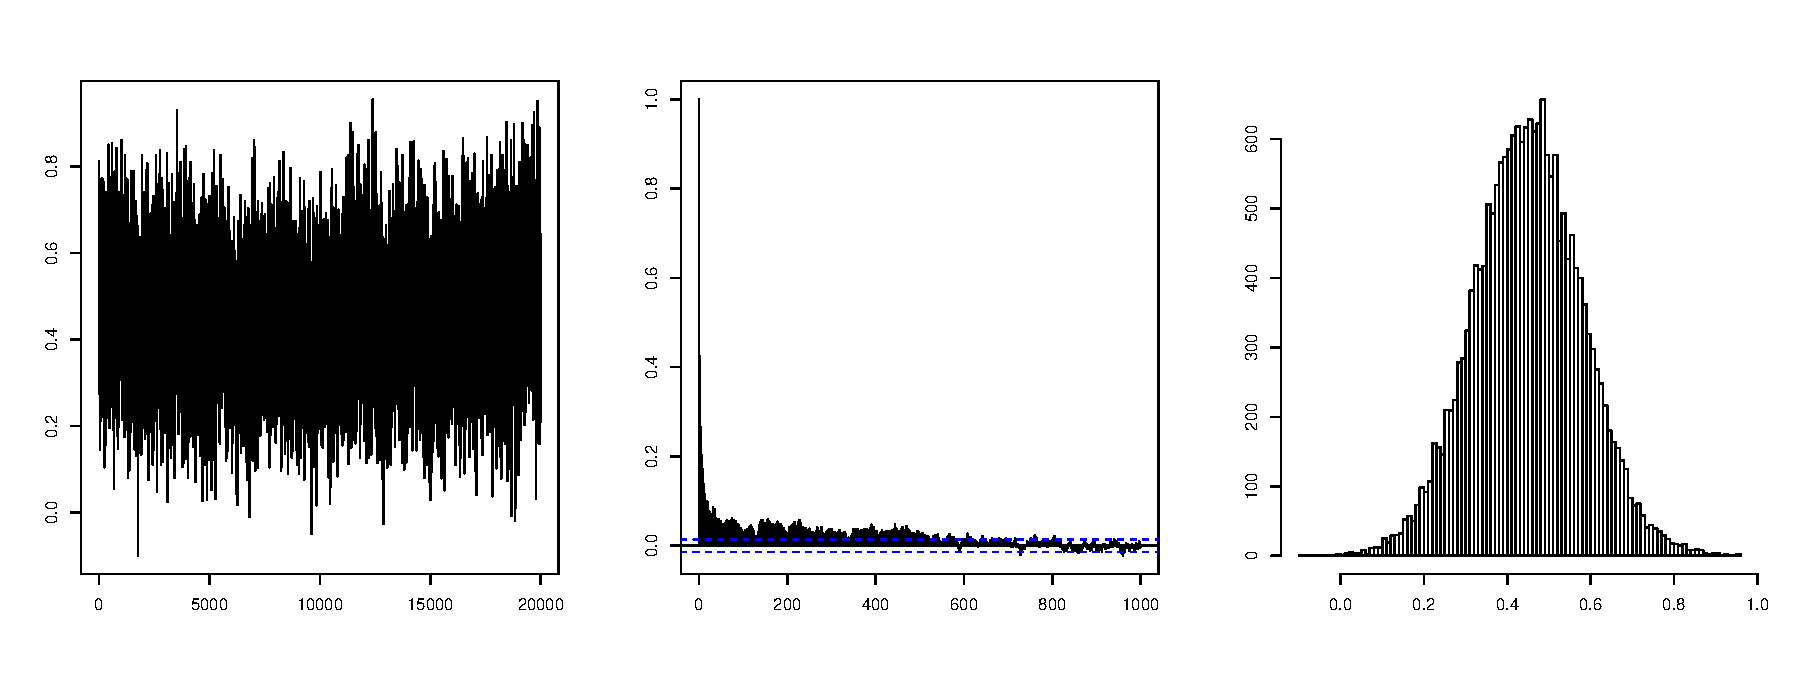
\includegraphics{bayesFAVAR_TVP_files/figure-latex/convergencePlot-1.pdf}
\caption{\label{fig:convergence}Kairėje 10000 parametro simuliacijų,
viduryje acf grafikas pirmam 1000 lagų, dešinėje posterioro simuliacijų
histograma}
\end{figure}

\begin{figure}[htbp]
\centering
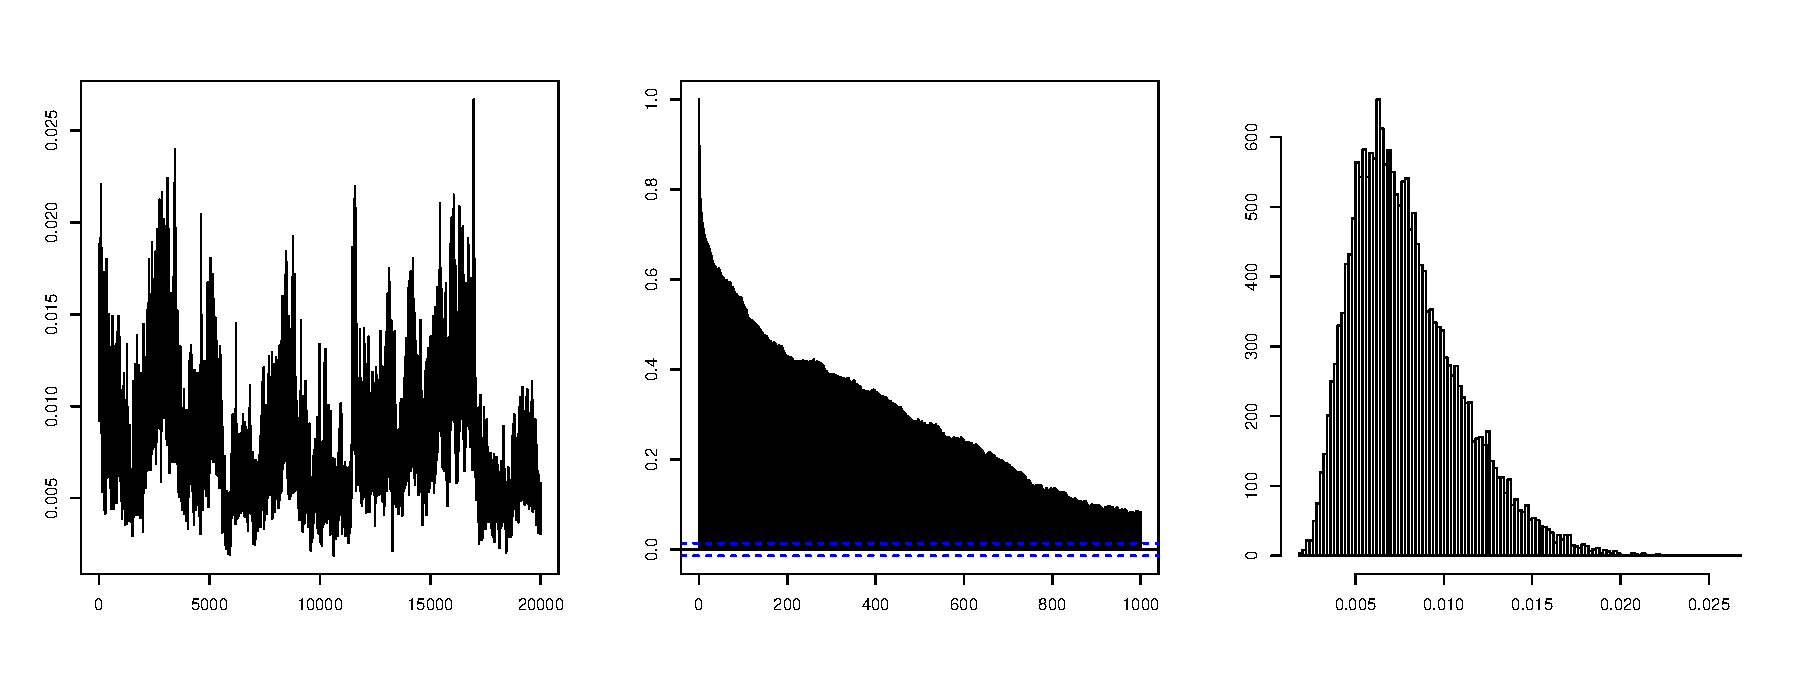
\includegraphics{bayesFAVAR_TVP_files/figure-latex/convergencePlot2-1.pdf}
\caption{\label{fig:convergence2}Kairėje 10000 parametro simuliacijų,
viduryje acf grafikas pirmam 1000 lagų, dešinėje posterioro simuliacijų
histograma}
\end{figure}

\subsection{Parametrų skirstiniai ir
įverčiai}\label{parametru-skirstiniai-ir-iverciai}

\ref{fig:beta_t} pav. pavaizduota beta posteriorų vidurkių kitimas
laike, o \ref{table:betaTable} lentelėje beta parametrų įverčiai
paskutiniam stebėtm periodui. Taip pat \ref{table:H} lentelėje pateikėme
H kovariacijų matricos parametrų posteriorų vidurkius. Dėl didelio
kiekio parametrų kiekio, vien iš jų sunku suprasti nagrinėjamų duomenų
eilučių sąryšius, todėl tokiais atvejais dažnai naudojama impulso-atsako
(angl. \emph{impulse-response}) funkcijos. 2016m. 4 ketv. jos
pavaizduotos \ref{fig:impulse-response} pav. Matome kai kuriuos
sąryšius, kurių ir buvo galima laukti. Pvz. infliacijos šokas paveikia
pajamingumų kreivę - didėja lygio (PC1) ir kreivumo (PC3) faktoriai, o
statumo (PC2) faktorius mažėja.

\begin{longtable}[]{@{}lrrrrrrr@{}}
\caption{\label{table:betaTable}Paskutinio periodo beta parametrų
įverčiai}\tabularnewline
\toprule
& const. & PC1\_L1 & PC2\_L1 & PC3\_L1 & UNRATE\_L1 & CPILFESL\_L1 &
GDPC1\_L1\tabularnewline
\midrule
\endfirsthead
\toprule
& const. & PC1\_L1 & PC2\_L1 & PC3\_L1 & UNRATE\_L1 & CPILFESL\_L1 &
GDPC1\_L1\tabularnewline
\midrule
\endhead
PC1 & 0.06 & 0.50 & 0.24 & 0.00 & 0.00 & 0.02 & -0.02\tabularnewline
PC2 & 0.11 & -0.02 & 0.67 & 0.04 & -0.01 & 0.01 & -0.03\tabularnewline
PC3 & 0.07 & 0.38 & -0.65 & 0.94 & 0.03 & 0.03 & -0.05\tabularnewline
UNRATE & 0.56 & -0.03 & 0.04 & 0.07 & 0.87 & 0.04 & -0.05\tabularnewline
CPILFESL & 1.11 & 0.87 & -0.80 & 0.22 & -0.11 & 0.64 &
-0.02\tabularnewline
GDPC1 & -0.70 & -0.61 & 0.64 & 0.02 & 0.28 & -0.23 & 0.75\tabularnewline
\bottomrule
\end{longtable}

\begin{longtable}[]{@{}lrrrrrr@{}}
\caption{\label{table:H}Kovariacijų matricos H įvertis}\tabularnewline
\toprule
& PC1 & PC2 & PC3 & UNRATE & CPILFESL & GDPC1\tabularnewline
\midrule
\endfirsthead
\toprule
& PC1 & PC2 & PC3 & UNRATE & CPILFESL & GDPC1\tabularnewline
\midrule
\endhead
PC1 & 0.03 & 0.01 & 0.02 & 0.00 & 0.00 & 0.03\tabularnewline
PC2 & 0.01 & 0.03 & 0.03 & 0.00 & 0.00 & 0.01\tabularnewline
PC3 & 0.02 & 0.03 & 0.14 & 0.00 & 0.01 & 0.06\tabularnewline
UNRATE & 0.00 & 0.00 & 0.00 & 0.03 & -0.01 & -0.05\tabularnewline
CPILFESL & 0.00 & 0.00 & 0.01 & -0.01 & 0.02 & 0.03\tabularnewline
GDPC1 & 0.03 & 0.01 & 0.06 & -0.05 & 0.03 & 0.67\tabularnewline
\bottomrule
\end{longtable}

\subsection{Prognozės ir scenarijų
analizė}\label{prognozes-ir-scenariju-analize}

Turint posterioro skirtinio simuliacijas gauti prognozių skirstinių
simuliacijas nesudėtinga. Įvertinus parametrus procesas toliau tesiamas
generuojant paklaidas pagal gautas kovariacijų matricas pasirinktą kiekį
periodų. Mes pasirinkome 4 periodų (vienų metų) horizontą.

Kaip minėjome užduoties aprašyme mus domina ne tik modelio implikuojma,
bet ir sąlyginė prognozė prie tam tikrų ekonomikos scenarijų. Šias
sąlygines prognozes randame ``pataisydami'' prognozės simuliacijas taip,
kad jų momentai tenkintų nurodytus apribojimus ir būtų kiek įmanoma
``arti'' pradinio simuliuoto skirstinio pagal Kullback-Leibler
informacijos kriterijų. Plačiau apie šį metodą galima rasti
\citet{Robertson2005}.

Savo analizėje suformavome tris ekonomikos scenarijus: optimistinį,
bazinį ir pesimistinį. Scenarijai suformuoti nurodant infliacijos,
nedarbo lygio ir RGDP vidurkius po metų. Scenarijai gali būti formuojami
įvariai, pvz. savo nuojauta ar ekonomistų prognozėmis. Mūsų suformuoti
scenarijai pateikiami \ref{table:economy_scenarios} lentelėje. Nagrinėtų
eilučių prognozių skirstiniai pateikiami \ref{fig:PredDensity} pav. ir
\ref{table:yc_forecast} lentelėje. \ref{fig:yc_forecast} pav. pateikiame
ir pačių pajamingumo kreivių prognozes. Gauti rezultatai intuityvūs:
gerėjant ekonominiai situacijai pajamingumų kreivė kyla į viršų, o
blogėjant atvirkščiai - pajamingumai mažėja.

\begin{longtable}[]{@{}lrrr@{}}
\caption{\label{table:economy_scenarios}Ekonominių duomenų raidos
scenarijai}\tabularnewline
\toprule
& UNRATE & CPILFESL & GDPC1\tabularnewline
\midrule
\endfirsthead
\toprule
& UNRATE & CPILFESL & GDPC1\tabularnewline
\midrule
\endhead
Optimistinis & 4.4 & 3.2 & 2.50\tabularnewline
Bazinis & 4.8 & 2.5 & 1.80\tabularnewline
Pesimistinis & 5.4 & 1.8 & 1.25\tabularnewline
\bottomrule
\end{longtable}

\begin{figure}[htbp]
\centering
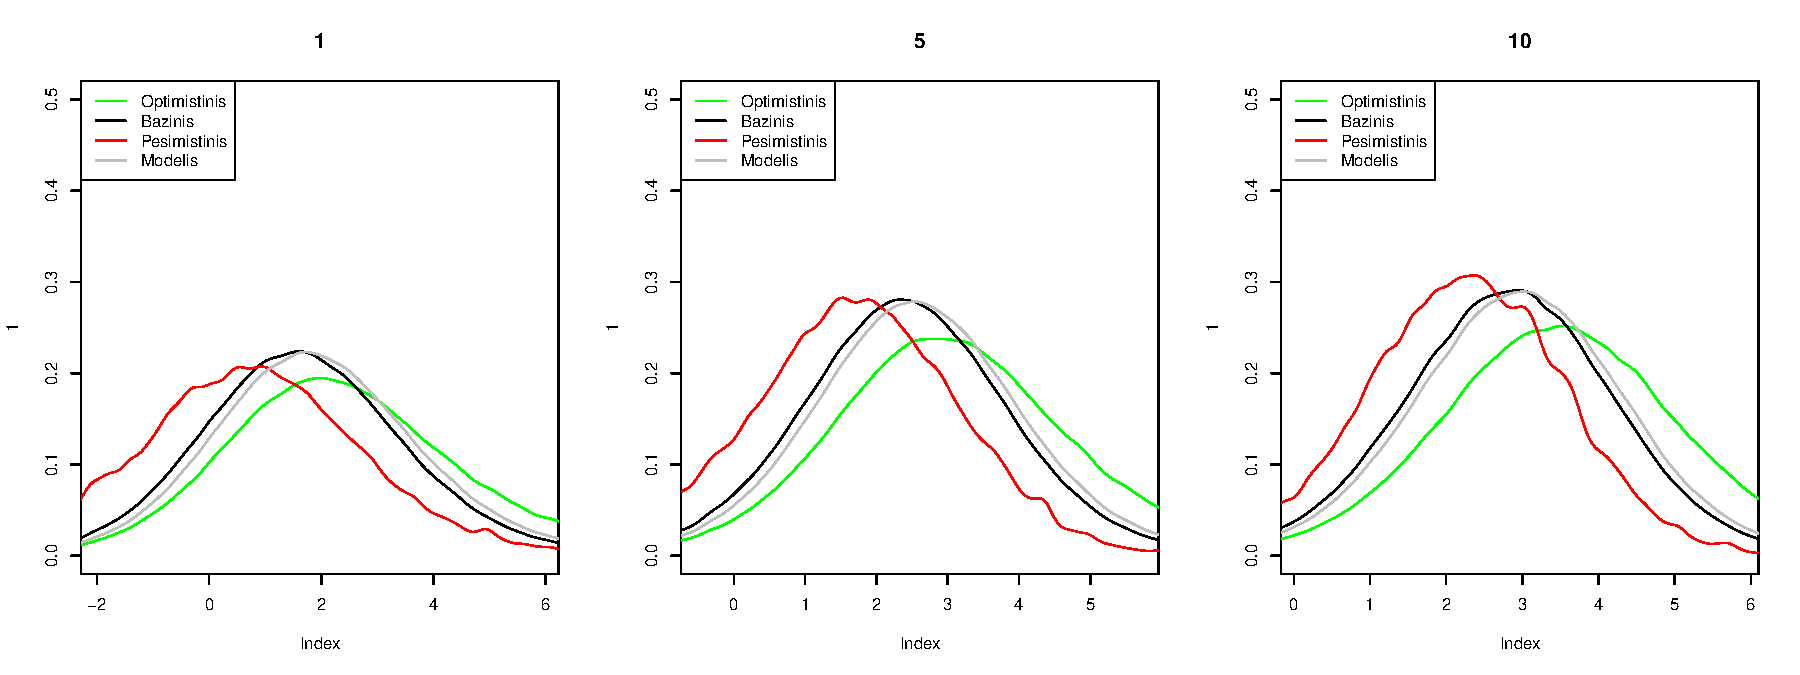
\includegraphics{bayesFAVAR_TVP_files/figure-latex/preddensity4-1.pdf}
\caption{\label{fig:PredDensity}Pajamingumų kreivės taškų sąlyginių
prognozių po 1 metų KDE tankiai skirtingais scenarijais}
\end{figure}

\begin{table}
\caption{\label{table:yc_forecast}Prognozės simuliacijų kvantiliai skirtingais scenarijais}

\centering
\begin{tabular}[t]{l|r|r|r|r|r}
\hline
\multicolumn{6}{c}{\textbf{Optimistinis}}\\
\hline
  & SVENPY01 & SVENPY03 & SVENPY05 & SVENPY07 & SVENPY10\\
\hline
5\% & -0.86 & -0.10 & 0.36 & 0.63 & 0.84\\
\hline
50\% & 2.34 & 2.76 & 3.06 & 3.29 & 3.51\\
\hline
95\% & 7.11 & 6.76 & 6.59 & 6.50 & 6.52\\
\hline
\end{tabular}
\centering
\begin{tabular}[t]{l|r|r|r|r|r}
\hline
\multicolumn{6}{c}{\textbf{Bazinis}}\\
\hline
  & SVENPY01 & SVENPY03 & SVENPY05 & SVENPY07 & SVENPY10\\
\hline
5\% & -1.31 & -0.52 & -0.04 & 0.24 & 0.45\\
\hline
50\% & 1.64 & 2.09 & 2.40 & 2.62 & 2.82\\
\hline
95\% & 4.94 & 4.89 & 4.91 & 4.98 & 5.12\\
\hline
\end{tabular}
\centering
\begin{tabular}[t]{l|r|r|r|r|r}
\hline
\multicolumn{6}{c}{\textbf{Pesimistinis}}\\
\hline
  & SVENPY01 & SVENPY03 & SVENPY05 & SVENPY07 & SVENPY10\\
\hline
5\% & -2.56 & -1.47 & -0.75 & -0.30 & -0.01\\
\hline
50\% & 0.73 & 1.32 & 1.71 & 2.00 & 2.25\\
\hline
95\% & 4.19 & 4.13 & 4.11 & 4.15 & 4.37\\
\hline
\end{tabular}
\centering
\begin{tabular}[t]{l|r|r|r|r|r}
\hline
\multicolumn{6}{c}{\textbf{Modelis}}\\
\hline
  & SVENPY01 & SVENPY03 & SVENPY05 & SVENPY07 & SVENPY10\\
\hline
5\% & -1.05 & -0.30 & 0.14 & 0.41 & 0.60\\
\hline
50\% & 1.88 & 2.29 & 2.57 & 2.77 & 2.97\\
\hline
95\% & 5.30 & 5.19 & 5.16 & 5.21 & 5.32\\
\hline
\end{tabular}
\end{table}

\begin{figure}[htbp]
\centering
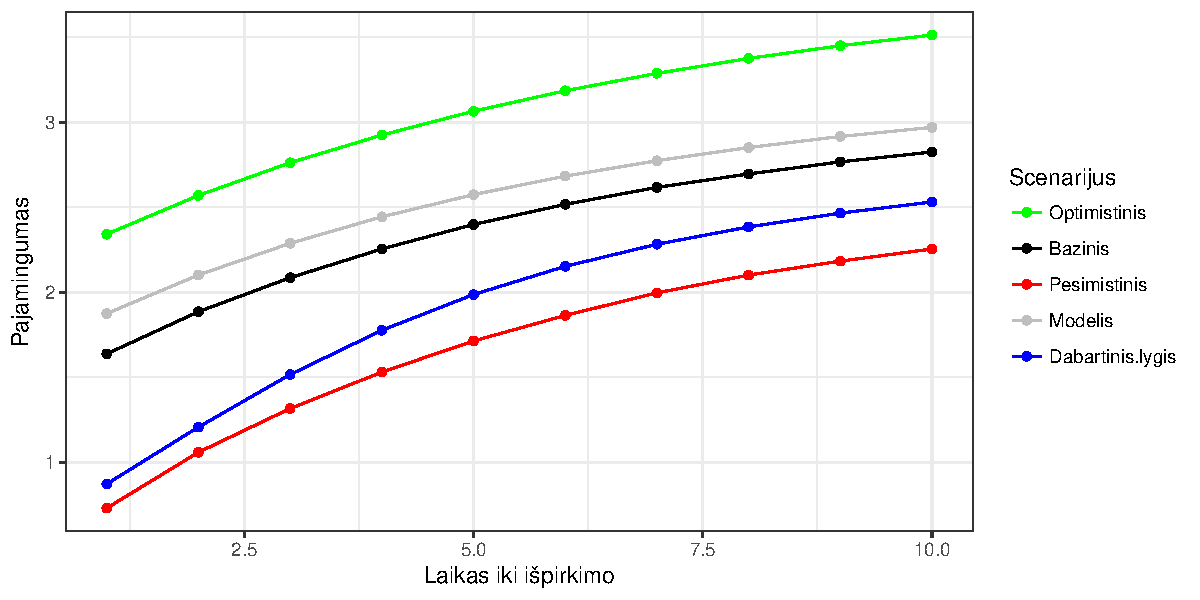
\includegraphics{bayesFAVAR_TVP_files/figure-latex/unnamed-chunk-11-1.pdf}
\caption{\label{fig:yc_forecast} Pajamingumo kreivės prognozės
(medianos) po 1 metų skirtingais ekonominiais scenarijais}
\end{figure}

\newpage

\section{Priedas. Paveikslėliai}\label{priedas.-paveiksleliai}

\begin{figure}[!htbp]

{\centering 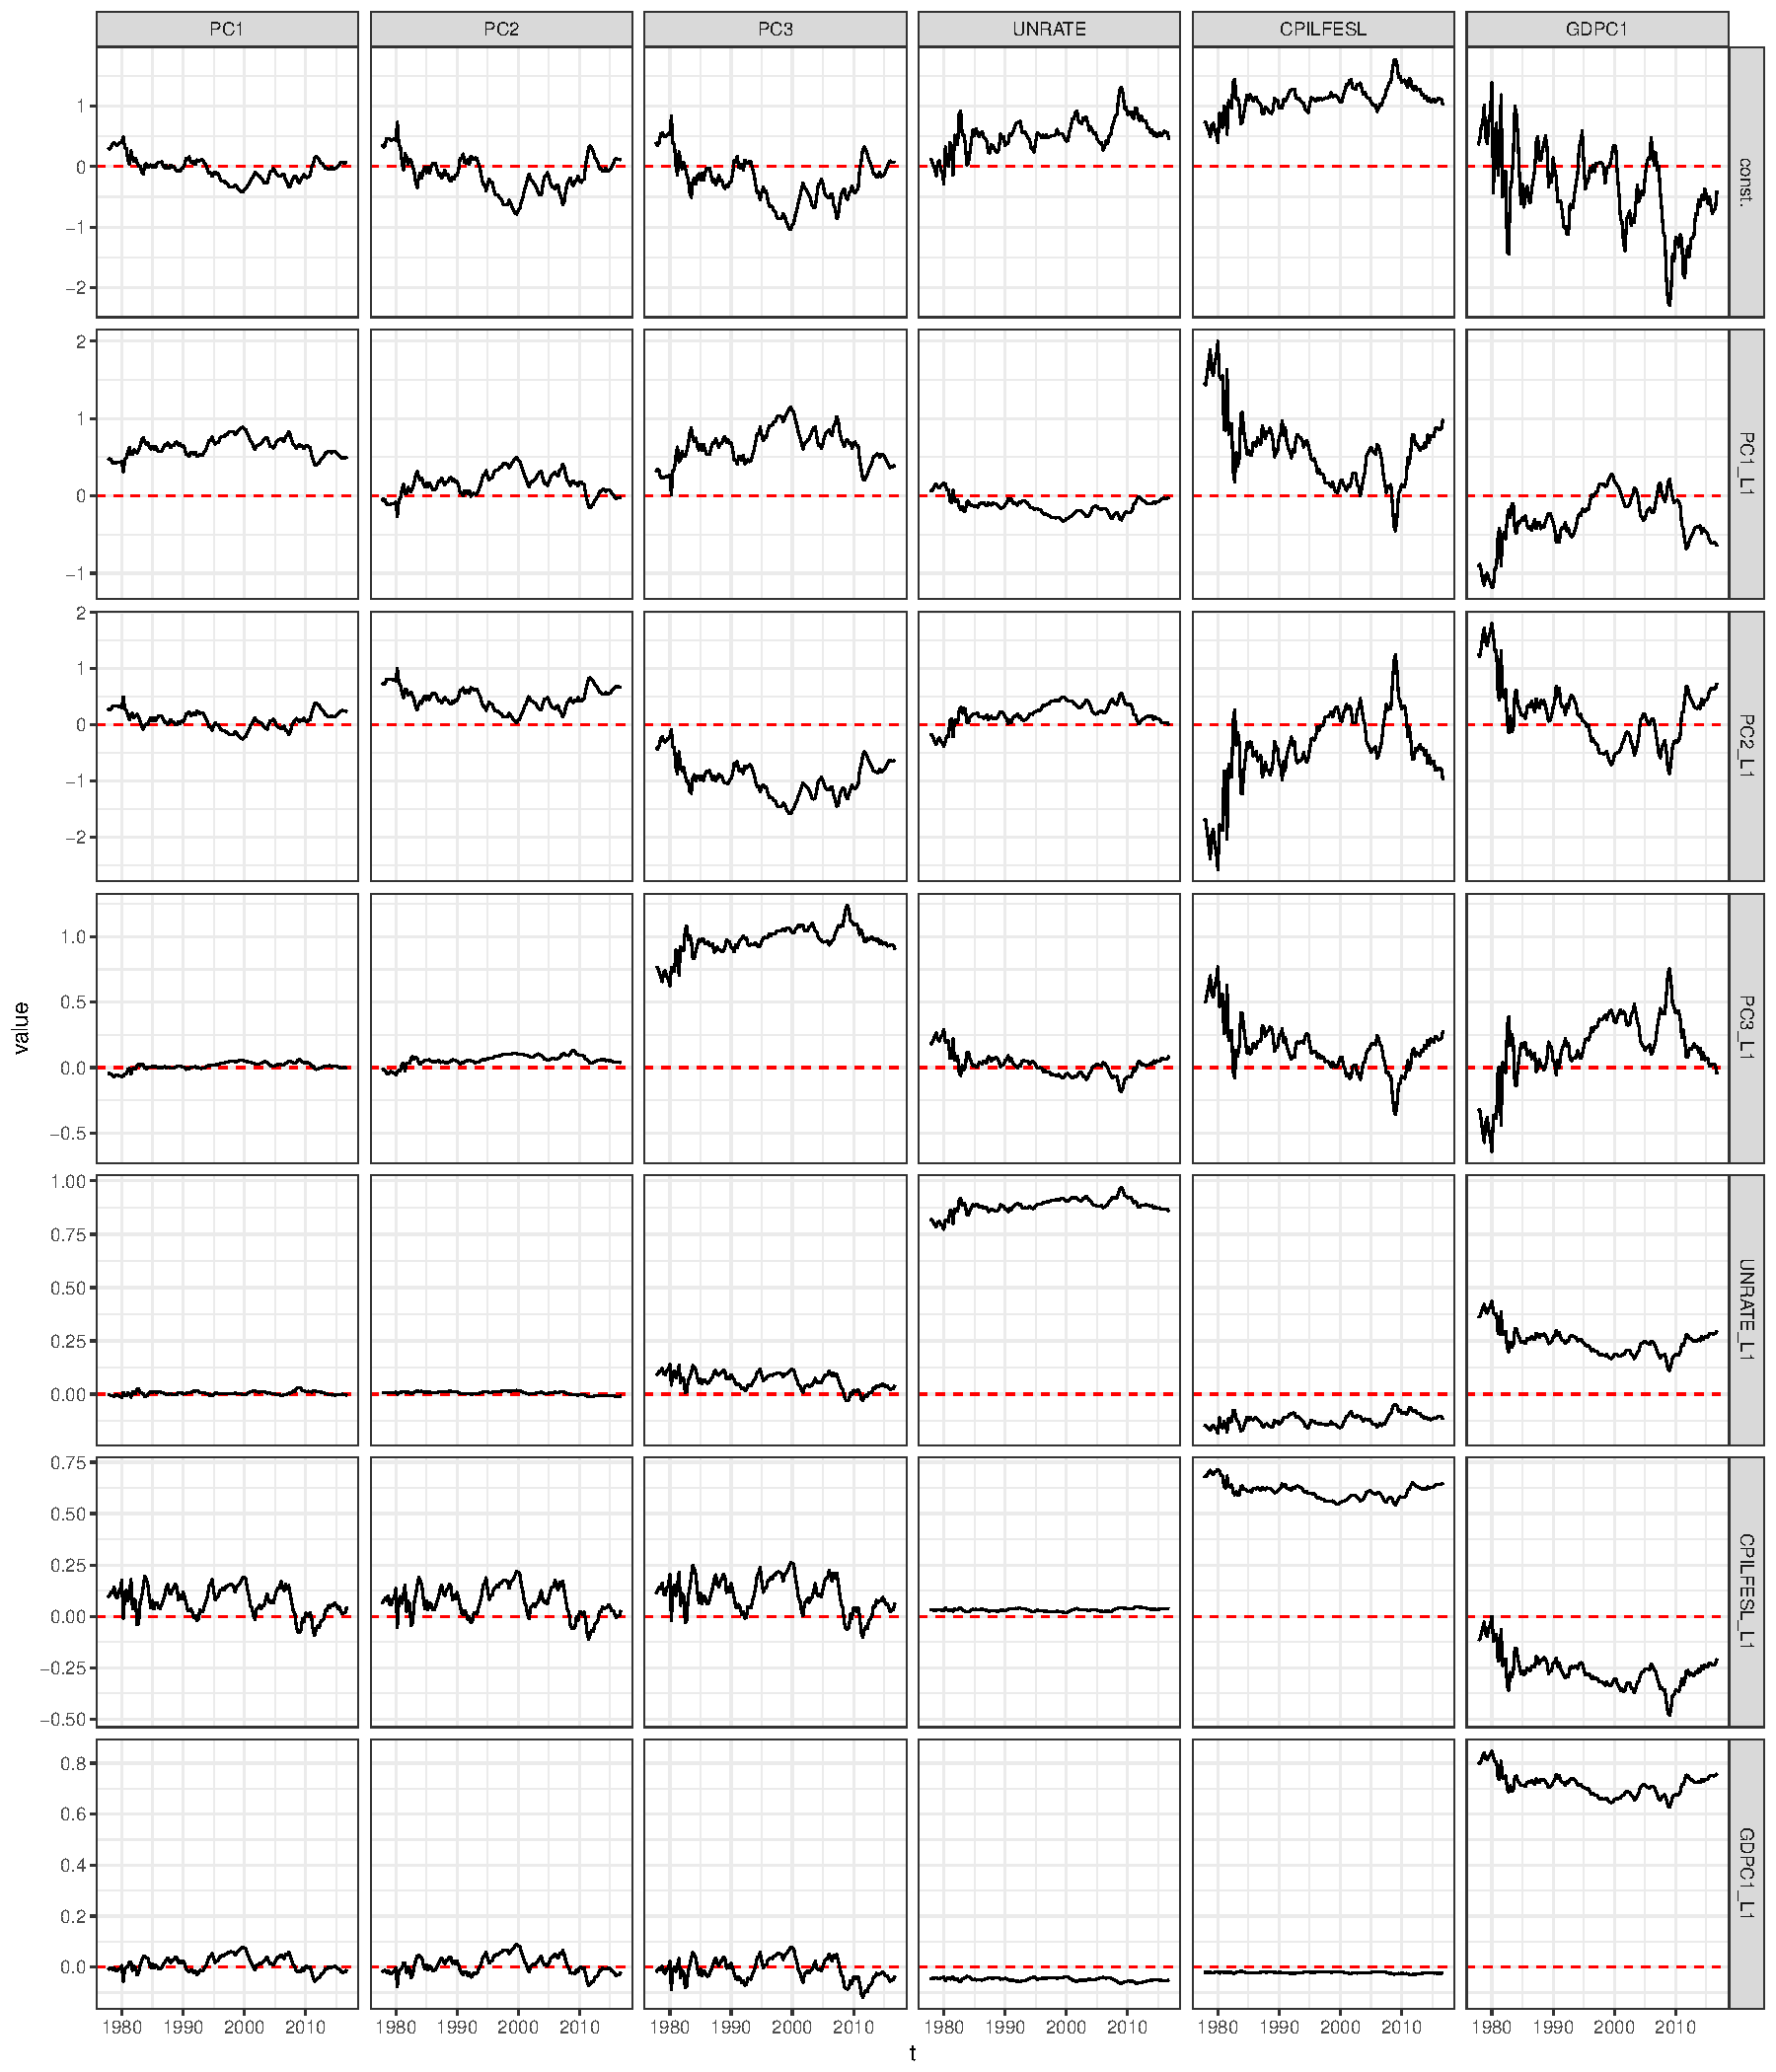
\includegraphics{bayesFAVAR_TVP_files/figure-latex/beta-1} 

}

\caption{\label{fig:beta_t}VAR-TVP(1) beta parametrų medianų kitimas laike}\label{fig:beta}
\end{figure}

\begin{figure}[htbp]
\centering
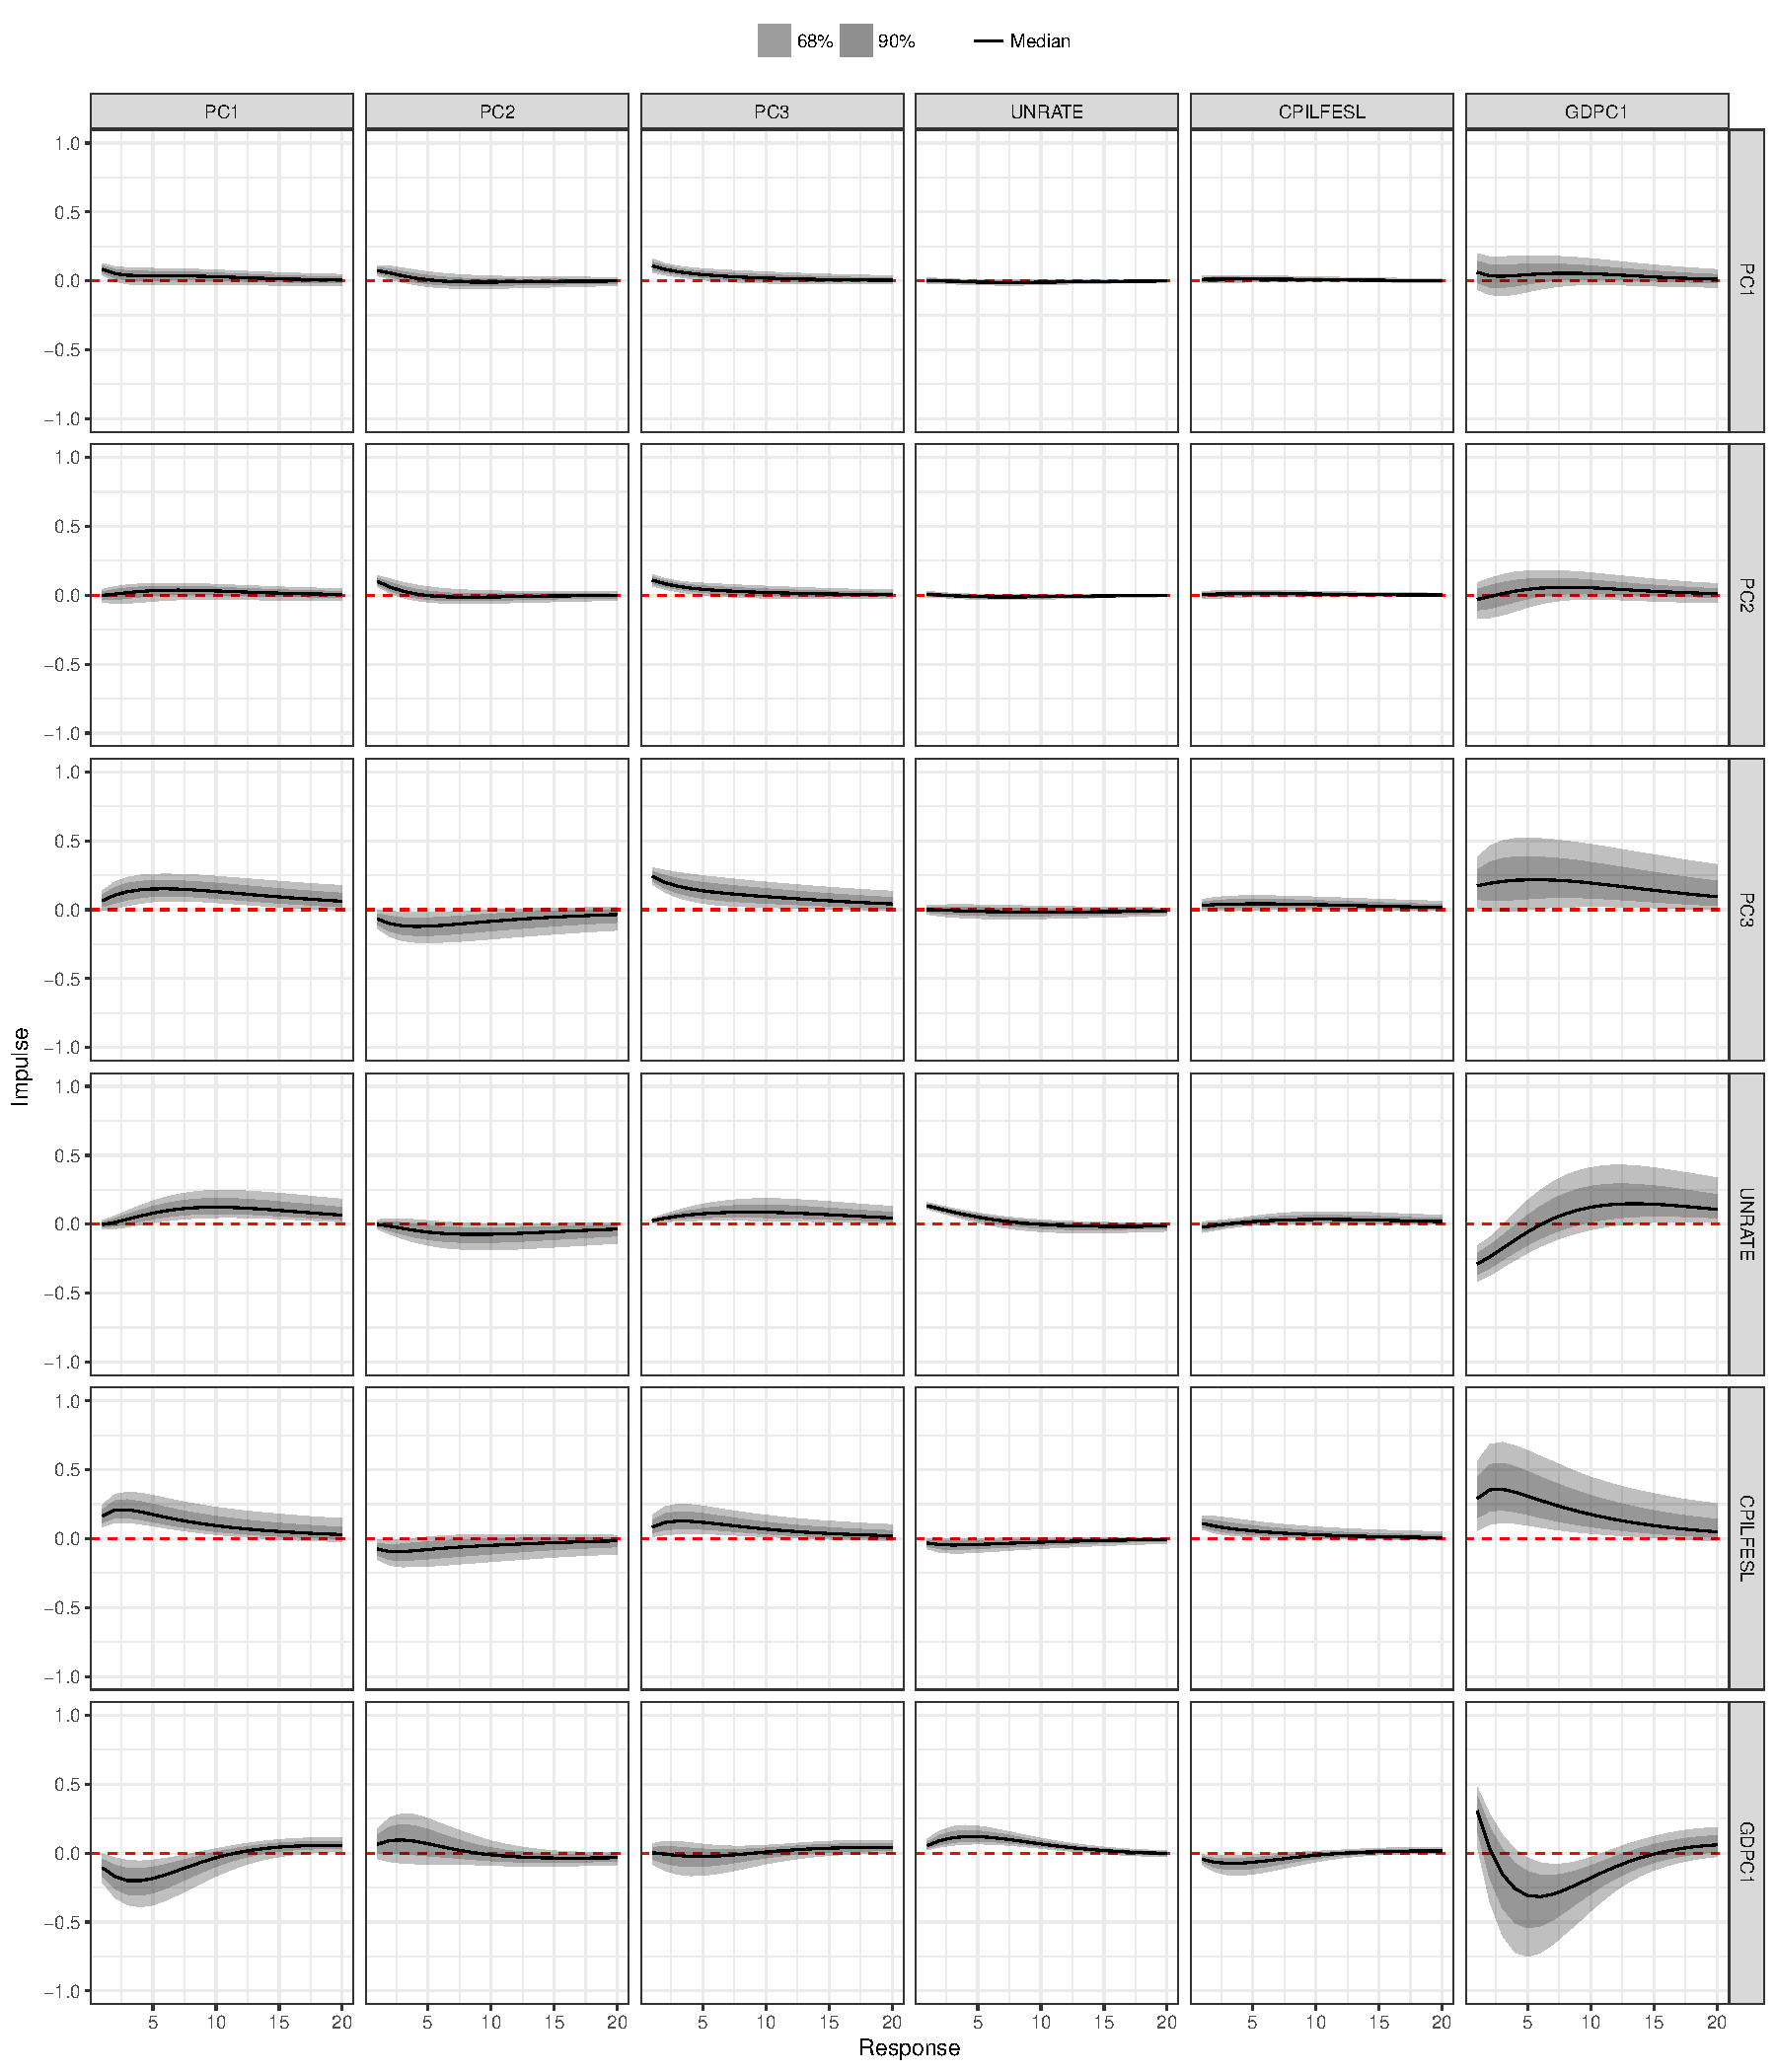
\includegraphics{bayesFAVAR_TVP_files/figure-latex/unnamed-chunk-13-1.pdf}
\caption{\label{fig:impulse-response}Impulso-atsako funkcijos 2016K3.
Horizontas 20 periodų (5 metai).}
\end{figure}

\section{Nuorodos į R/C++ kodą}\label{nuorodos-i-rc-koda}

Pagrindinė dalis kodo sudėta į \texttt{bayesVAR\_TVP} paketą. Jį galima
rasti: \url{https://github.com/GediminasB/bayesVAR_TVP}. Pačios
ataiskaitos \texttt{Rmarkdown} kodas ir naudoti duomenys čia:
\url{https://github.com/GediminasB/MIF_bayesVAR_tyrimas}

\renewcommand\refname{Literatūros sąrašas}
\bibliography{references}


\end{document}
